\documentclass[DIN, pagenumber=false, fontsize=11pt, parskip=half]{scrartcl}

\usepackage{ngerman}
\usepackage[utf8]{inputenc}
\usepackage[T1]{fontenc}
\usepackage{textcomp}
\usepackage{amsmath}
\usepackage{amsfonts}
\usepackage{tikz}

% for matlab code
% bw = blackwhite - optimized for print, otherwise source is colored
\usepackage[framed,numbered,bw]{styles/exercise}

% for other code
%\usepackage{listings}

\setlength{\parindent}{0em}

% set section in CM
\setkomafont{section}{\normalfont\bfseries\Large}

\newcommand{\mytitle}[1]{{\noindent\Large\textbf{#1}}}
\newcommand{\mysection}[1]{\textbf{\section*{#1}}}
\newcommand{\mysubsection}[2]{\romannumeral #1) #2}


%===================================
\begin{document}

\noindent\textbf{Very Deep Learning} \hfill \textbf{Technische Universität Kaiserslautern} \\
WS 2022/23 \hfill Dr. Muhammad Zeshan Afzal \\

\mytitle{Exercise 1 - Computational Graphs and Gradients}

\textbf{Deadline: 14.11.2022 \hfill Total Marks: 30}


\section*{Submission}

\begin{itemize}
    \item All submissions will be handled through OLAT.
    \item Your submission should contain a PDF with the solutions to the exercise questions (and any Python code files) zipped together in a single file.
    \item Include the group number along with the names and matriculation numbers of all group members on the PDF.
    \item For Jupyter notebook, please save it with the outputs of your code displayed.
    \item The points obtained in the bonus exercise will only be added to your total if the total does not exceed the exercise total. You can see this as a way of making up for any points lost in the other sections.
\end{itemize}

%===================================
\mysection{1.1. Basics\hfill[1+1+1+1+1=5]}

\mysubsection{1}{What is deep learning? What makes a neural network ,,deep''?}

\mysubsection{2}{What do you understand by the term backpropagation?}

\mysubsection{3}{Why do we use activation functions in neural networks?}

\mysubsection{4}{What is the difference between supervised and unsupervised learning?}

\mysubsection{5}{What is a Tensor in PyTorch and how is it different from a matrix?}



%===================================
\mysection{1.2. Computational Graphs\hfill[3+3+2+4=12]}

Computational graphs are directed graphs that represent the dependencies between the variables and operations within a model or, more generally, a mathematical expression. As an example, give the expression \[f(w, x, y, z) = 4(xyz + max(z, w))\] it has the following computational graph:

\begin{figure}[h!]
\centering
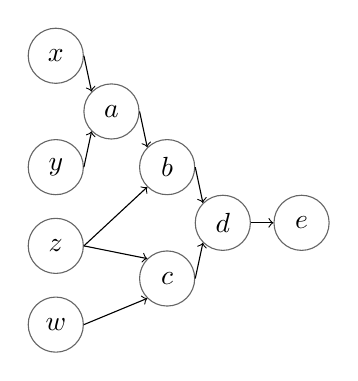
\begin{tikzpicture}[
roundnode/.style={circle, draw=black!60, fill=white!0, minimum size=7mm},
]
%Nodes
\node[roundnode]      (e)       [] {$e$};
\node[roundnode]      (d)       [left of=e] {$d$};
\node[roundnode]      (c)       [below left of=d] {$c$};
\node[roundnode]      (b)       [above left of=d] {$b$};
\node[roundnode]      (a)       [above left of=b] {$a$};
\node[roundnode]      (x)       [above left of=a]{$x$};
\node[roundnode]      (y)       [below left of=a] {$y$};
\node[roundnode]      (z)       [below of=y] {$z$};
\node[roundnode]      (w)       [below of=z] {$w$};

%Lines
\draw[->] (x.east) -- (a.north west);
\draw[->] (y.east) -- (a.south west);
\draw[->] (a.east) -- (b.north west);
\draw[->] (z.east) -- (b.south west);
\draw[->] (z.east) -- (c.north west);
\draw[->] (w.east) -- (c.south west);
\draw[->] (b.east) -- (d.north west);
\draw[->] (c.east) -- (d.south west);
\draw[->] (d.east) -- (e.west);
\end{tikzpicture}
\end{figure}

where $a = xy$, $b = az = xyz$, $c = max(z, w)$, $d = b + c$ and $e = 4d$.

\textbf{Tasks:} Now, consider the following expressions:
\begin{align*}
\begin{split}
    \mathcal{A} &= (a - (b \cdot c)) \cdot d \\
    \mathcal{B} &= \sqrt{a + b + c^3} + \log(\frac{a}{d}) \\
    \mathcal{C} &= d - \exp^{(a + b) \cdot c}
\end{split}
\end{align*}

\mysubsection{1}{Introduce intermediate variables \textbf{for all three expressions} such that each variable represents a single mathematical operation.}

\mysubsection{2}{Using your chosen intermediate variables, draw computational graphs \textbf{for all three expressions}.}

\mysubsection{3}{Given that $a=2$, $b=-7$, $c=4$ and $d=1$. Perform forward propagation on \textbf{any two} of the three computational graphs you created in (ii).}

\mysubsection{4}{Perform backpropagation on the \textbf{same two} computational graphs you chose in (iii).}


%===================================
\mysection{1.3. Vanishing and Exploding Gradients \hfill [1+3+2+1+3=10]}

Consider a network with input $x \in \mathbb{R}$, 4 hidden layers each having only one node, and one output $y \in \mathbb{R}$:

\begin{figure}[h]
\centering
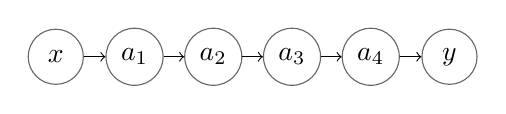
\begin{tikzpicture}[
roundnode/.style={circle, draw=black!60, fill=white!0, minimum size=7mm},
]
%Nodes
\node[roundnode]      (x)       [] {$x$};
\node[roundnode]      (a1)      [right of=x] {$a_1$};
\node[roundnode]      (a2)      [right of=a1] {$a_2$};
\node[roundnode]      (a3)      [right of=a2] {$a_3$};
\node[roundnode]      (a4)      [right of=a3] {$a_4$};
\node[roundnode]      (y)       [right of=a4] {$y$};

%Lines
\draw[->] (x.east) -- (a1.west);
\draw[->] (a1.east) -- (a2.west);
\draw[->] (a2.east) -- (a3.west);
\draw[->] (a3.east) -- (a4.west);
\draw[->] (a4.east) -- (y.west);
\end{tikzpicture}
\end{figure}

In the network each node corresponds to the sigmoid of the preceding node multiplied with some weight:
$a_i = \sigma(w_i \cdot a_{i-1})$, $i = 1, \ldots 5$, where $a_0$ corresponds to the input $x$ and $a_5$ corresponds to the output $y$.

The sigmoid function is given by \[\sigma(x) = \frac{1}{1 + e^{-x}}\]

\textbf{Tasks:}

\mysubsection{1}{What is the vanishing gradients problem?}

\mysubsection{2}{Calculate the derivative $\sigma'$ of the sigmoid function. What are the minimum and maximum values of the derivative?}

\mysubsection{3}{By using the chain rule, calculate the gradient $\frac{\partial{y}}{\partial{x}}$.}

\mysubsection{4}{Does the maximum value of the derivative of sigmoid contribute to the vanishing gradients problem? If so, how?}

\mysubsection{5}{What is meant by exploding gradients? Why do we not want the gradients to explode? When can sigmoid activations have an exploding gradient?}


%===================================
\mysection{1.4. Handwritten Digit Recognition Using PyTorch\hfill[3]}

Follow the instructions in the Jupyter notebook \texttt{exercise\_1.ipynb} to perform handwritten digit recognition using PyTorch. The notebook contains detailed instructions about downloading the dataset, creating the neural network, training it, and evaluating the results.

Your task is to fill in the missing code annotated with \texttt{TODO} tags in the comments. You can get up to 3 points if you can fill in all the missing code, successfully train the network and get an accuracy of around 90\% on the test data.

\textbf{As a bonus exercise, if you can do modifications to the network architecture or the training parameters such that you can get an accuracy above 95\%, you can get 2 additional points.}

\textit{Hint: You can import the notebook in Google Colab to get started with minimal setup or to use GPUs.}

\end{document}